\documentclass{standalone}
\usepackage{pgfplots}
\pgfplotsset{compat=1.18}
\usepgfplotslibrary{groupplots,fillbetween}
\begin{document}
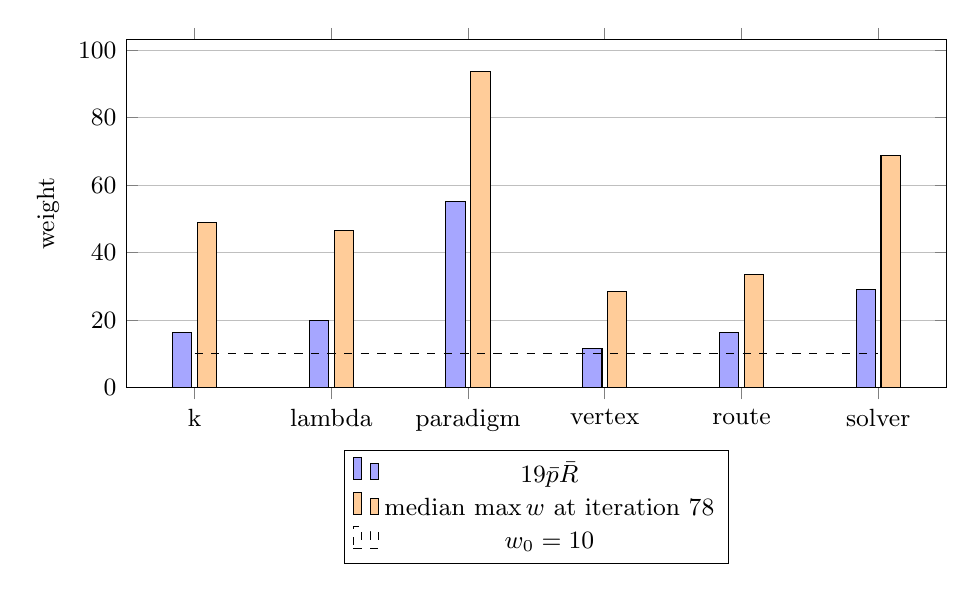
\begin{tikzpicture}
\begin{axis}[
  ybar,
  bar width=7pt,
  width=12cm, height=6cm,
  symbolic x coords={k,lambda,paradigm,vertex,route,solver},
  xtick=data,
  ylabel={weight},
  ymin=0,
  tick label style={font=\small},
  label style={font=\small},
  legend style={font=\small, at={(0.5,-0.18)}, anchor=north},
  ymajorgrids,
  clip=false,
]
\addplot[fill=blue!35, draw=black] coordinates {(k, 16.2702) (lambda, 19.9851) (paradigm, 55.2362) (vertex, 11.6063) (route, 16.3092) (solver, 29.1894)};
\addlegendentry{$19\bar p\bar R$}
\addplot[fill=orange!40, draw=black] coordinates {(k, 48.9385) (lambda, 46.4636) (paradigm, 93.7180) (vertex, 28.4998) (route, 33.5958) (solver, 68.6967)};
\addlegendentry{median $\max w$ at iteration 78}
\addlegendimage{black, dashed}
\addlegendentry{$w_0=10$}
\draw[dashed] (axis cs:k,10) -- (axis cs:solver,10);
\end{axis}
\end{tikzpicture}
\end{document}
